\chapter{Results $\&$ Discussion}
\section{$v_2$ Measurement}
The resulting $v_2$ measurement for p+Au @ $\sqrt{s}$ 200 GeV $0-5\%$ centrality shown in \ref{fig:pau_points_alone}. There is a significant $v_2$, even in a small system such as p+Au.

%\subsection{$v_2$ vs $p_T$}
\begin{figure}
\begin{center}
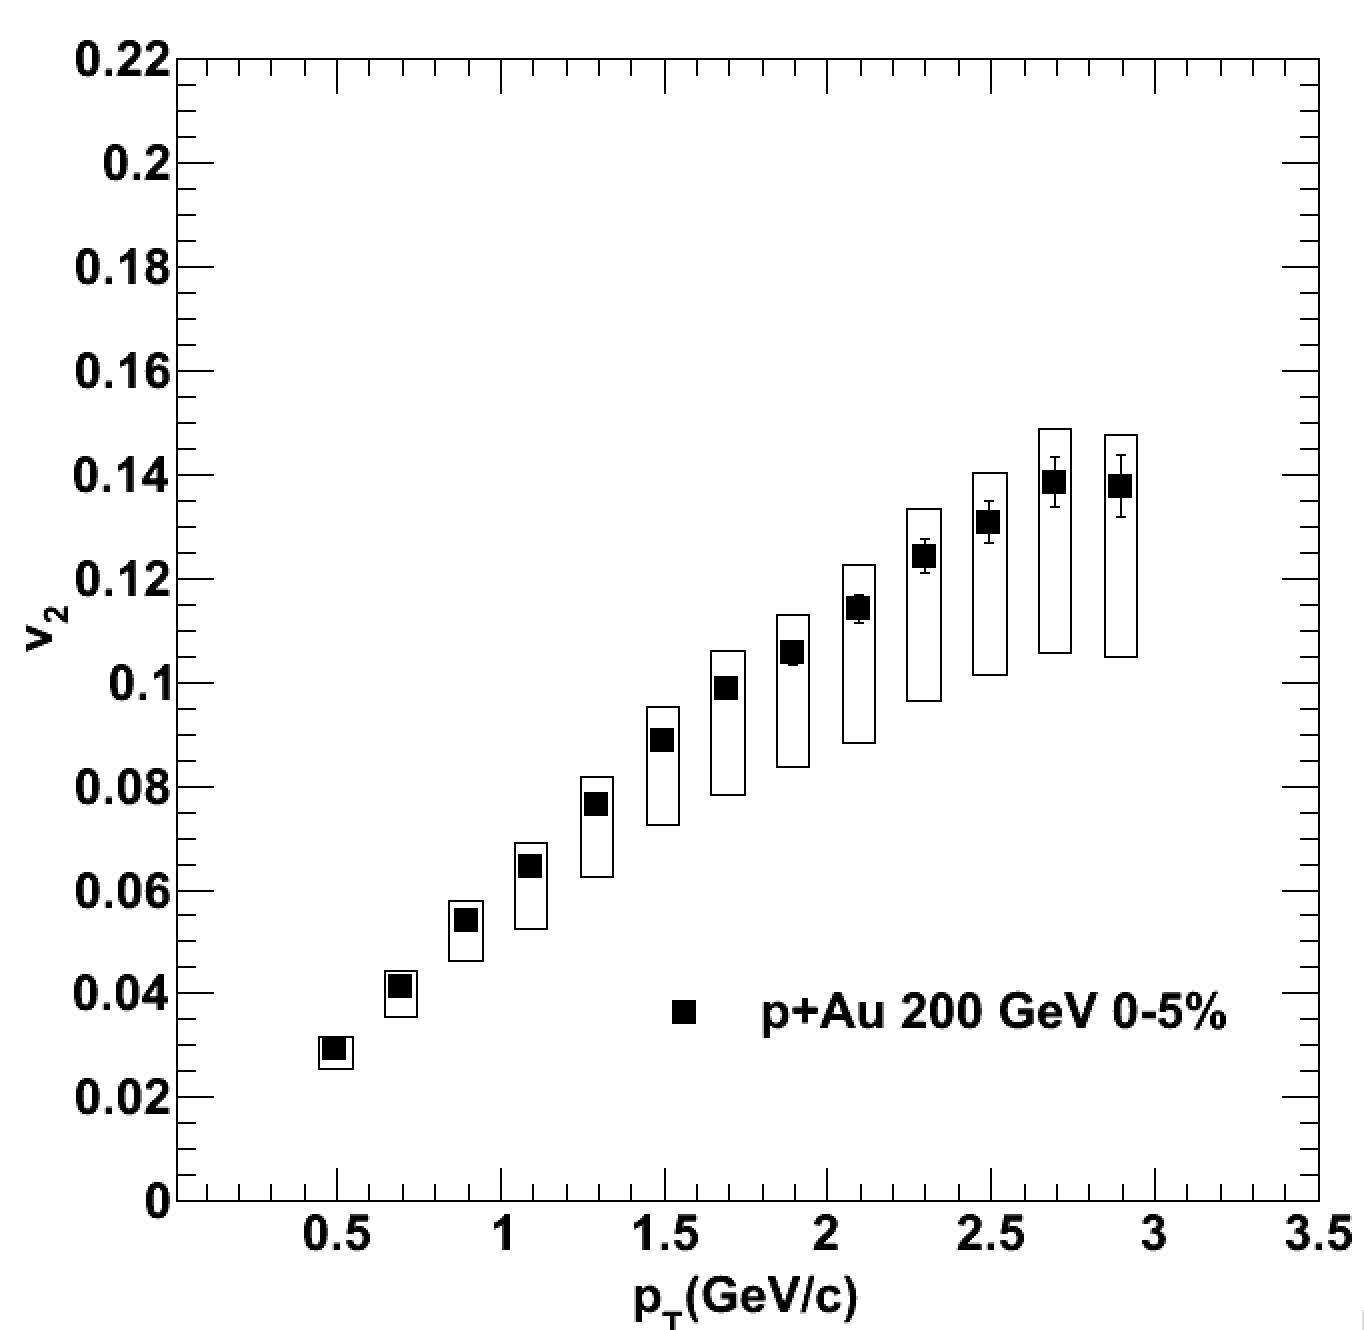
\includegraphics[width=0.75\linewidth]{figs/pau_points.png}
\caption{The $v_2$ measurement of p+Au @ $\sqrt{s}$ 200 GeV $0-5\%$ centrality. Statistical and systematic errors are shown. The systematic errors are very large especially at high $p_t$ and are dominated by non-flow.}
\label{fig:pau_points_alone}
\end{center}
\end{figure}
%\subsection{$v_2$ vs Multiplicity}

\section{Comparison with Theory}
\subsection{SONIC}
Also shown in Fig. ~\ref{fig:hydro_pau_alone} are $v_2$ calculations for each system from the \textsc{sonic} hydrodynamic model~\cite{Habich:2014jna}, which incorporates standard Monte Carlo Glauber initial conditions followed by viscous hydrodynamics with $\eta/s=0.08$, and a transition to a  hadronic cascade at $T=$ 170 MeV. It is notable that these calculations for each system are matched to the charged particle density at midrapidity, with the exact values for $0\%-5\%$ centrality of 10.0, 20.0, and 27.0, for p+Au, d+Au, and He+Au collisions, respectively~\cite{Habich:2014jna}. Again, note that $dN_{cn}/d\eta$ has not been measured for p+Au, and that the value of 10.0 was extrapolated from measurements in the other two systems~\cite{Habich:2014jna}. We thus see that the calculation includes both the geometry-related change in eccentricity and the relative collision multiplicity. In all cases, a good agreement is seen within uncertainties between the data and the calculation. These observations strongly support the notion of initial geometry, coupled to the hydrodynamic evolution of the medium as a valid framework to understand small system collectivity.

\begin{figure}
\begin{center}
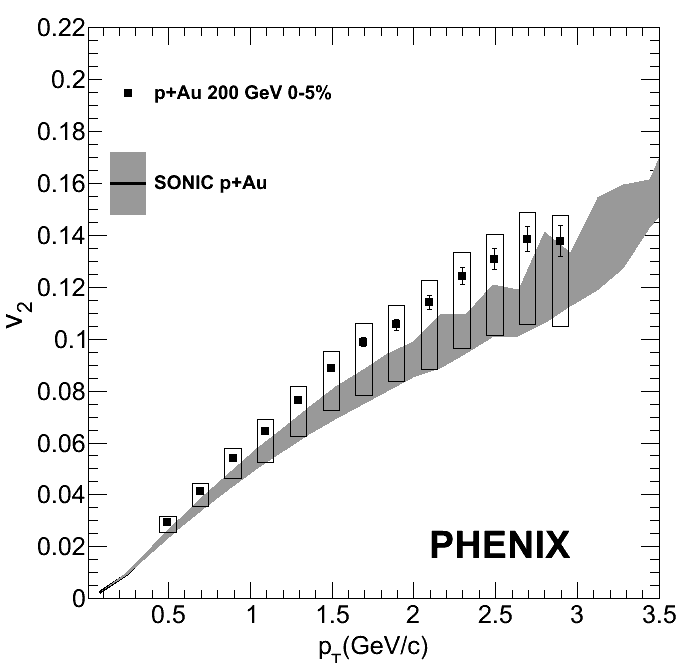
\includegraphics[width=0.75\linewidth]{figs/pau_sonic_alone.png}
\caption{$v_2$ of charged hadrons within $|\eta| <$ 0.35 in 0\%--5\% p+Au compared to calculations using the \textsc{sonic} model match to the same multiplicity as the data. The model calculations have good agreement with the center of the systematic uncertainty bars.}
\label{fig:hydro_pau_alone}
\end{center}
\end{figure}

\section{Comparison with Other Species}

\begin{figure}
\begin{center}
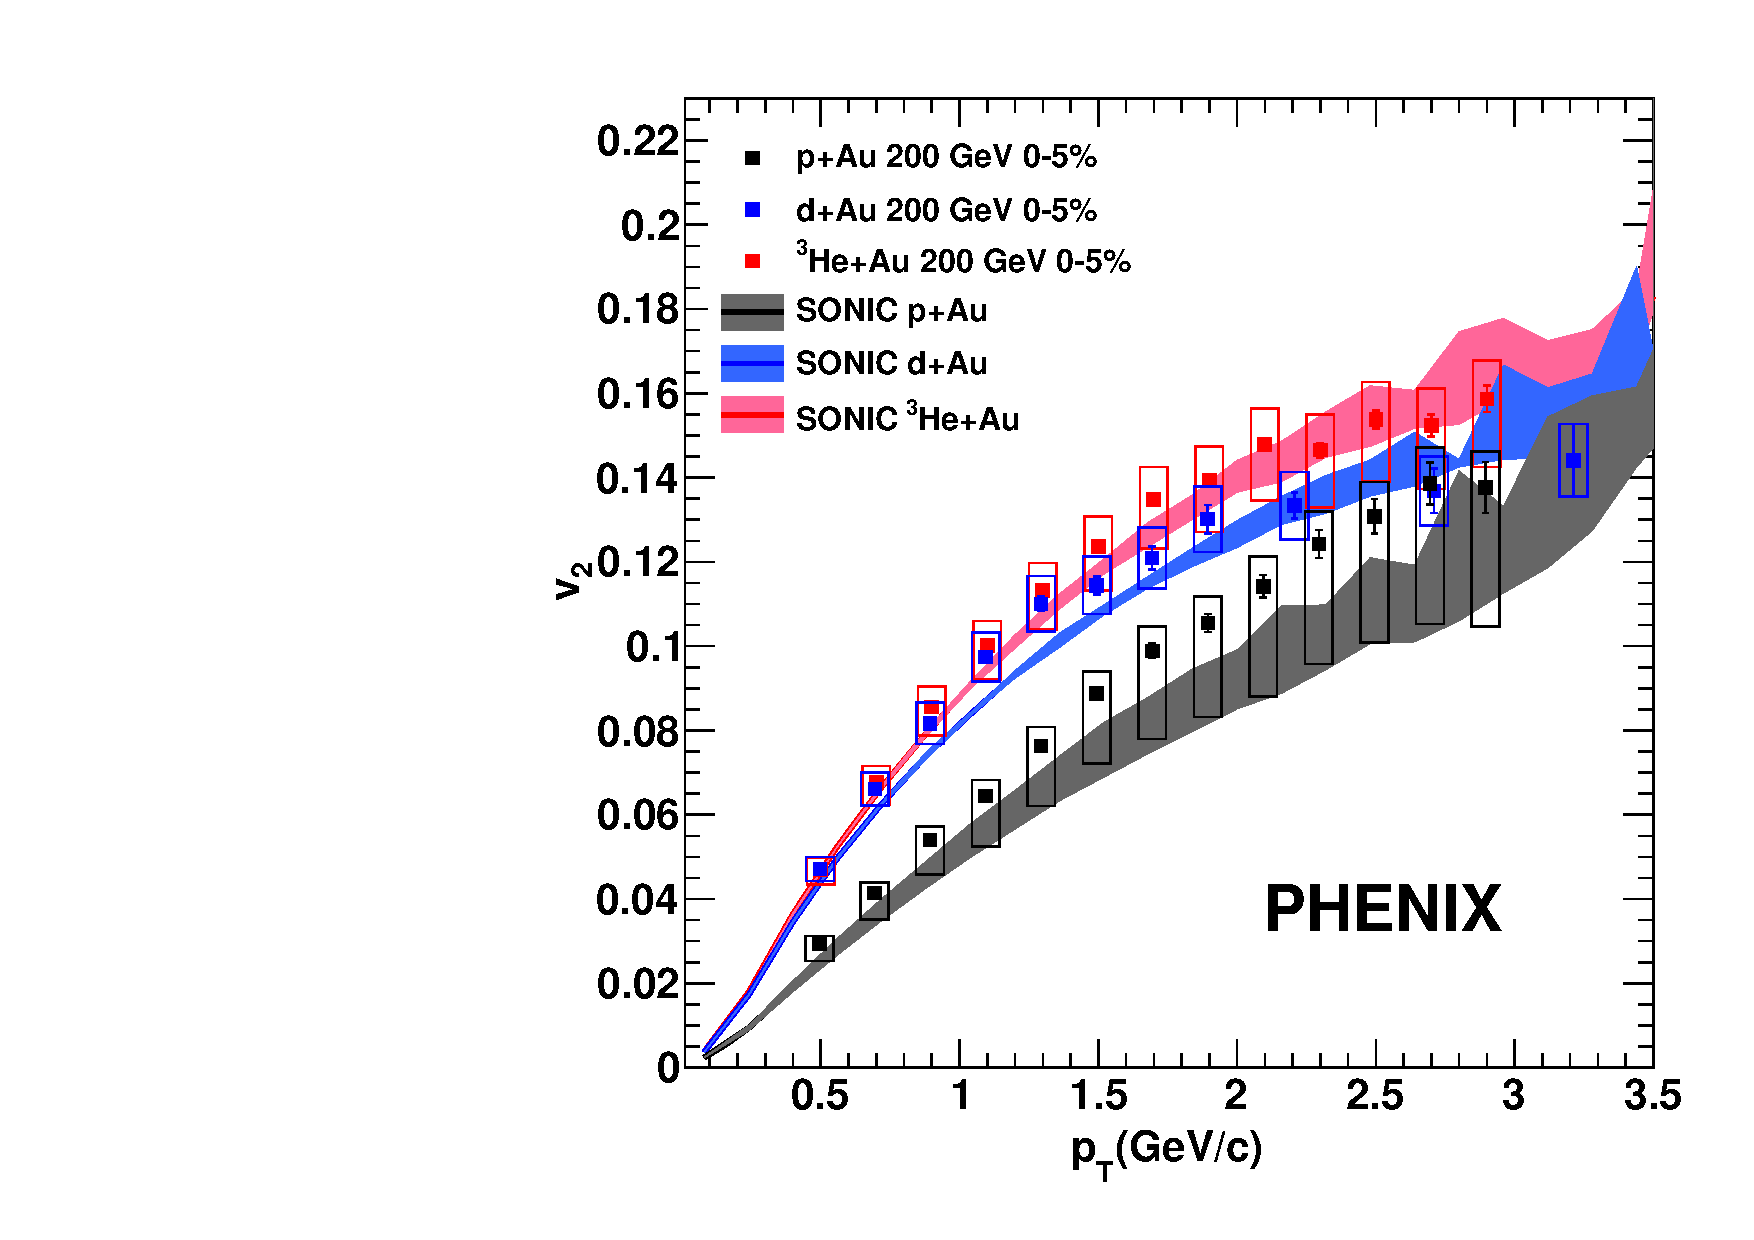
\includegraphics[width=0.5\linewidth]{figs/three_system_comparison_result.pdf}
\caption{$v_2$ of charged hadrons within $|\eta| <$ 0.35 in 0\%--5\% p+Au, d+Au, and HeAu central collisions, compared to hydrodynamic calculations using the \textsc{sonic} model, matched to the same multiplicity as the data. Note that the data points shown include non-flow contributions, whose estimated magnitude is accounted for in the asymmetric systematic uncertainties.}
\label{fig:all_system_hydro}
\end{center}
\end{figure}

\begin{figure}
\begin{center}
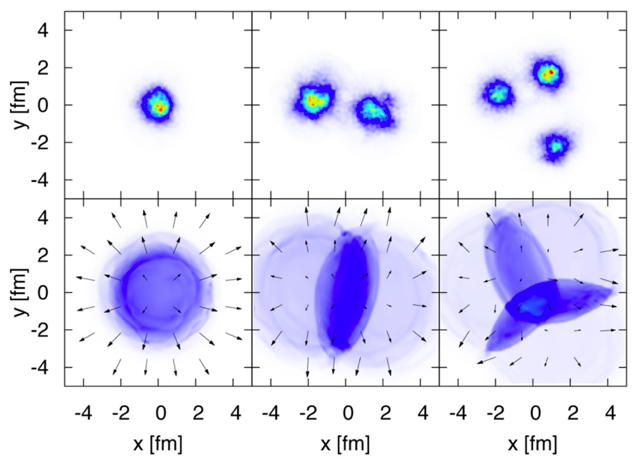
\includegraphics[width=0.75\linewidth]{figs/initial_condition_comparison.png}
\caption{TBA}
\label{fig:initial_condition_comparison}
\end{center}
\end{figure}
We can compare the p+Au $v_2$ measurement compared to d+Au
[add ref] %~\cite{Adare:2014keg} 
and He+Au
%~\cite{Adare:2015ctn} 
[add ref]
in the same $0\%-5\%$ centrality class, is shown in Fig.~\ref{fig:all_system_hydro}. The d+Au data, as presented in Ref.
%~\cite{Adare:2014keg}
[add ref], did not include non-flow contributions in its systematic uncertainties, which are now accounted for in the systematics shown in Fig.~\ref{fig:all_system_hydro}. In all cases, there is a substantial $v_2$ that rises with $p_T$. It is notable that the $v_2$ values for d+Au and He+Au are consistent within uncertainties, as are their eccentricities $\varepsilon_2$ listed in Table \ref{table_geometry_glasma}. The p+Au collisions have a significantly lower $v_2$ and a correspondingly lower calculated $\varepsilon_2$. At the same time, the ordering of $v_2$ from p+Au, to d+Au, to He+Au also follows the expected increasing order of particle multiplicity. In the case of d+Au and He+Au, for the $0\%-5\%$ most central events, the published values for midrapidity charged particle density are $dN_{ch}/d\eta$ = 20.8 $\pm$ 1.5 and 26.3 $\pm$ 1.8, respectively
%~\cite{Adare:2015bua}
[add ref]. This quantity has not yet been measured in p+Au collisions.
\begin{table}[h!]
\caption{Initial eccentricity $\varepsilon_2$ of small systems at $\sqrt{s}$ = 200 GeV for $0\%-5\%$ centrality from Monte Carlo Glauber initial conditions smeared with a two-dimensional Gaussian of width $\sigma=0.4$ fm, and IP-Glasma initial conditions.}
\begin{tabular}{c c c c}
\label{table_geometry_glasma}
 & p+Au & d+Au & He+Au \\ \hline
 Glauber $\langle \varepsilon_2 \rangle$ & $0.23\pm 0.01$ & $0.54\pm 0.04$ & $0.50\pm 0.02$ \\
 IP-Glasma $\langle \varepsilon_2 \rangle$ & $0.10\pm 0.02$ & $0.59\pm 0.01$ & $0.55\pm 0.01$ \\
\end{tabular}
\end{table}

\subsection{AMPT}
Finally, \textsc{ampt} combines partonic and hadronic scattering in a single model. Central \textsc{ampt} events with impact parameter $b<2$ have a midrapidity $dN_{ch}/d\eta$ = 8.1, 14.8, and 20.7 for p+Au, d+Au, and \hau, respectively. These were generated with the same Monte Carlo Glauber initial conditions used to characterize event geometry, and thus have very similar eccentricities to those given in Table I. Using the initial Glauber geometry information to compute $v_2$ relative to the participant plane~\cite{Koop:2015wea} yields results that agree reasonably well with the data below $\pt \approx 1$ GeV/c, yet underpredict them at higher \pt. It is noteworthy that despite the very different physics of \textsc{ampt} compared to the other models, it has successfully been applied to a variety of systems at RHIC and the LHC. See, for example, Refs.~\cite{Adare:2015cpn,Koop:2015wea,Ma:2016fve,ma_long-range_2014,ma_long-range_2014}

\begin{figure}
\begin{center}
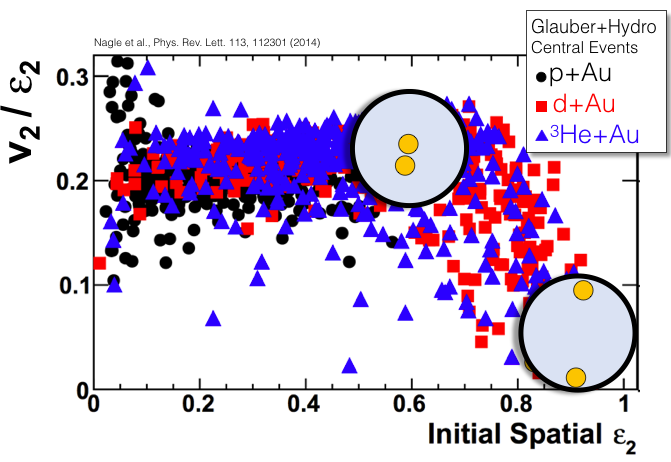
\includegraphics[width=0.6\linewidth]{figs/v2_e2_ampt.png}
\caption{TBA}
\end{center}
\end{figure}
\subsection{IP-Glasma with Hydro}
\begin{figure}
\begin{center}
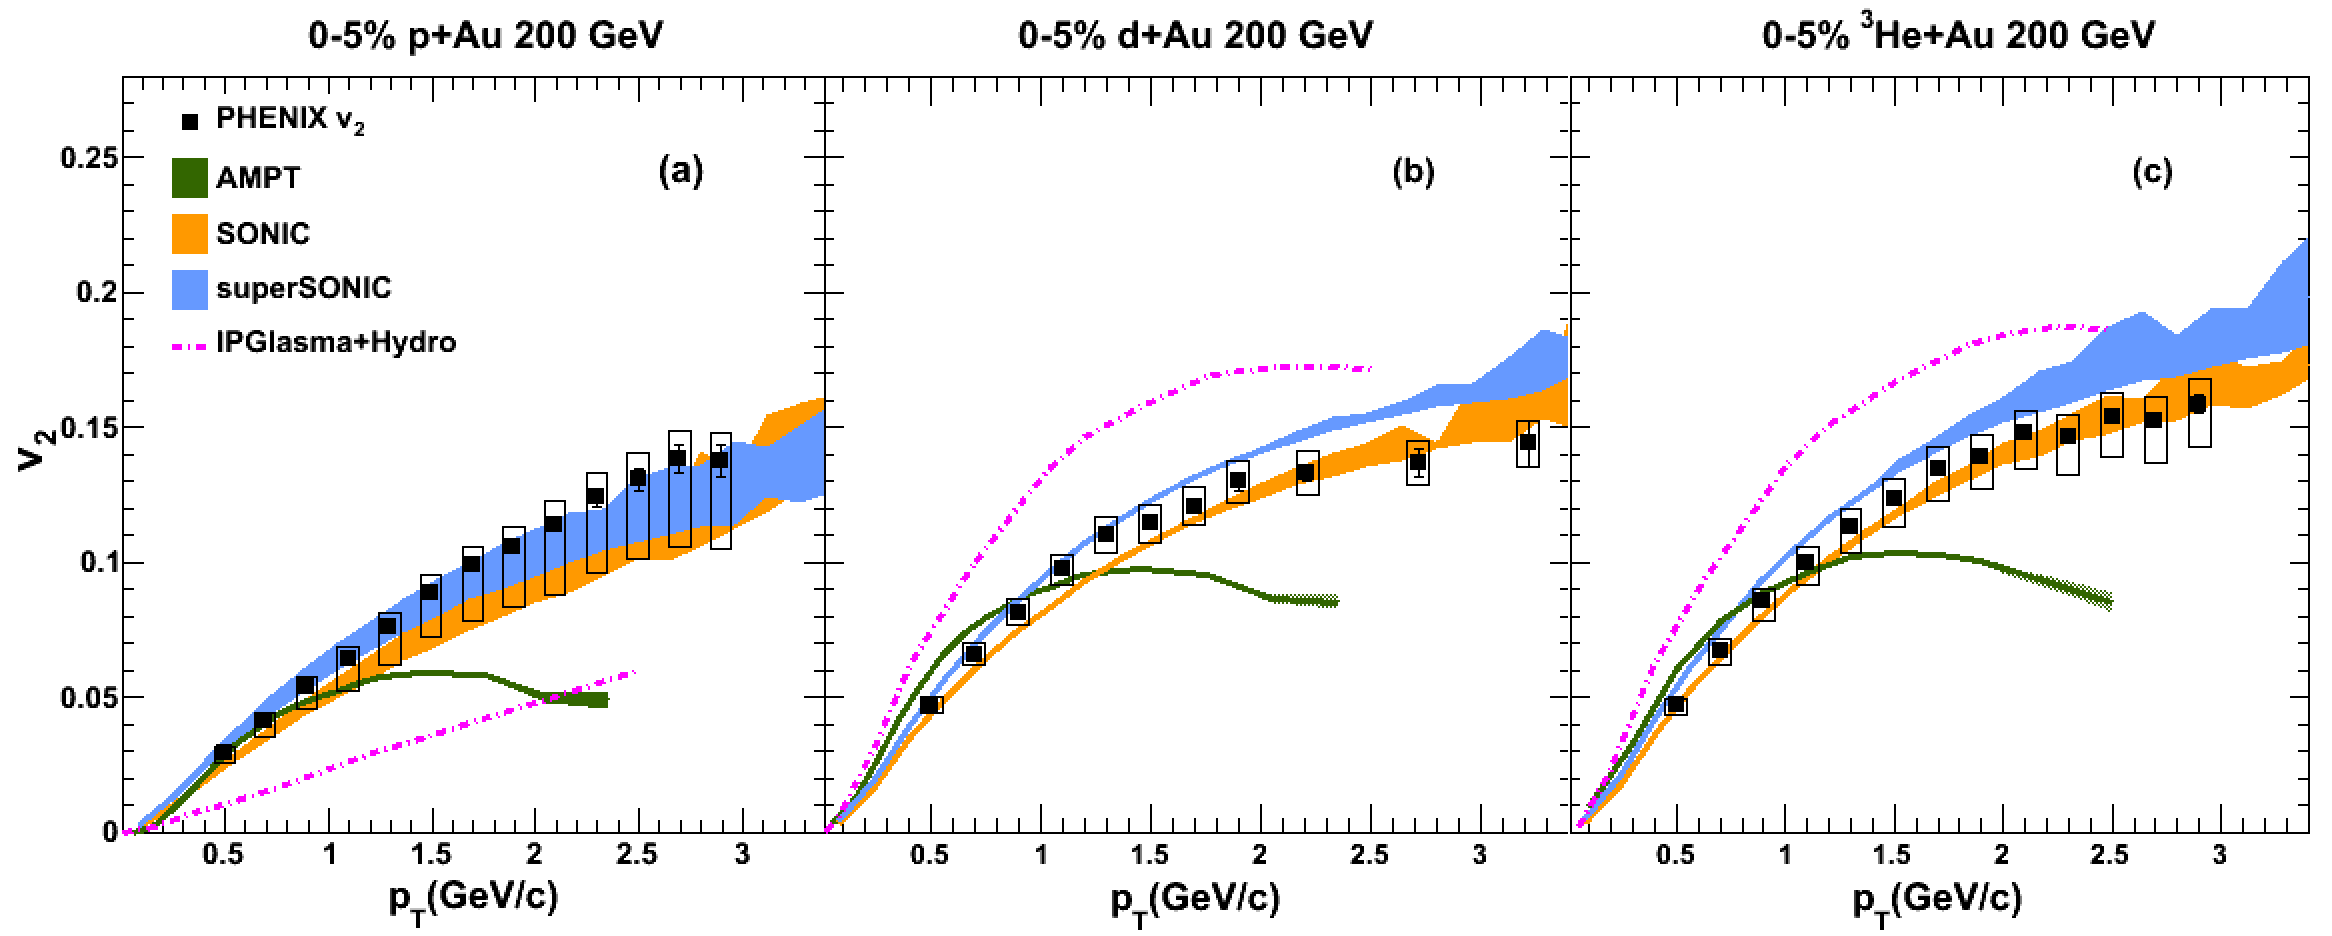
\includegraphics[width=0.9\linewidth]{figs/indepth_theory_comparison.png}
\caption{Transverse momentum dependence of $v_2$ in central 0\%-5\% (a) p+Au, (b) d+Au, and (c) He+Au collisions at $\sqrt{s}$ = 200 GeV. Theoretical calculations from \textsc{ampt}, \textsc{(super)sonic}, and IPGlasma+Hydro are shown in each panel. Note that the data points shown include non-flow contributions, whose estimated magnitude is accounted for in the asymmetric systematic uncertainties.}
\end{center}
\end{figure}
